\documentclass[12pt,1p]{elsarticle}
\usepackage{amsmath}
\usepackage{amssymb}
%usepackage{epsfig}
\usepackage{graphicx}
\usepackage{array}
\biboptions{sort&compress}
\usepackage{url}
\def\UrlBreaks{\do\/\do-}

% *** GRAPHICS RELATED PACKAGES ***
%
%\ifCLASSINFOpdf
%  % \usepackage[pdftex]{graphicx}
%  % declare the path(s) where your graphic files are
%  % \graphicspath{{../pdf/}{../jpeg/}}
%  % and their extensions so you won't have to specify these with
%  % every instance of \includegraphics
%  % \DeclareGraphicsExtensions{.pdf,.jpeg,.png}
%\else
%  % or other class option (dvipsone, dvipdf, if not using dvips). graphicx
%  % will default to the driver specified in the system graphics.cfg if no
%  % driver is specified.
%  \usepackage[dvips]{graphicx}
%  % declare the path(s) where your graphic files are
%  % \graphicspath{{../eps/}}
%  % and their extensions so you won't have to specify these with
%  % every instance of \includegraphics
%  % \DeclareGraphicsExtensions{.eps}
%\fi


%%%%%%%%%%%%%%%\hyphenation{op-tical net-works semi-conduc-tor}
\newcommand{\sgn}{\mathrm{sign} \:}

\begin{document}

\begin{frontmatter}
	
	%% Title, authors and addresses
	
	%% use the tnoteref command within \title for footnotes;
	%% use the tnotetext command for theassociated footnote;
	%% use the fnref command within \author or \address for footnotes;
	%% use the fntext command for theassociated footnote;
	%% use the corref command within \author for corresponding author footnotes;
	%% use the cortext command for theassociated footnote;
	%% use the ead command for the email address,
	%% and the form \ead[url] for the home page:
	%% \title{Title\tnoteref{label1}}
	%% \tnotetext[label1]{}
	%% \author{Name\corref{cor1}\fnref{label2}}
	%% \ead{email address}
	%% \ead[url]{home page}
	%% \fntext[label2]{}
	%% \cortext[cor1]{}
	%% \address{Address\fnref{label3}}
	%% \fntext[label3]{}
	
	\title{Tutoring math platform accessible for visually impaired people}
	
	%% use optional labels to link authors explicitly to addresses:
	%% \author[label1,label2]{}
	%% \address[label1]{}
	%% \address[label2]{}
	
	\author{Michał Sebastian Maćkowski, Piotr Franciszek Brzozaa}
	\address{Computer Science Department, Silesian University of Technology, 16 Akademicka, 44-100 Gliwice, Poland}
		
	\author{Dominik Roland Spinczykb}
	\address{Biomedical Engineering Department, Silesian University of Technology, 40 Roosevelta, 41-800 Zabrze, Poland}
	
	\begin{abstract}
	
	Background: There are many problems with
teaching and assessing impaired students in higher education,
especially in technical science, where the knowledge is
represented mostly by structural information like: math
formulae, charts, graphs, etc. Developing e-learning platform for
distance education solves this problem only partially due to the
lack of accessibility for the blind.

	Method: The proposed method is based on the decomposition
of the typical mathematical exercise into a sequence of
elementary sub-exercises. This allows for interactive resolving of
math exercises and assessment of the correctness of exercise
solutions at every stage. The presented methods were prepared
and evaluated by visually impaired people and students.

	Results: The article presents the accessible interactive
tutoring platform for math teaching and assessment, and
experience in exploring it. The results of conducted research
confirm good understanding of math formulae described
according to elaborated rules. Regardless of the level of
complexity of the math formulae the level of math formulae
understanding is higher for alternative structural description.

	Conclusions: The proposed solution enables alternative
descriptions of math formulae. Based on the research results, the
tool for computer-aided interactive learning of mathematics
adapted to the needs of the blind has been designed, implemented
and deployed as a platform for on-site and online and distance
learning. The designed solution can be very helpful in
overcoming many barriers that occur while teaching impaired
students.
	\end{abstract}
	
	\begin{keyword}
		%% keywords here, in the form: keyword \sep keyword
		Assistive technology\sep Education for people with special needs\sep Visually impaired people\sep Alternative presentation of math structural information
		%% PACS codes here, in the form: \PACS code \sep code
		
		%% MSC codes here, in the form: \MSC code \sep code
		%% or \MSC[2008] code \sep code (2000 is the default)
		
	\end{keyword}
	
\end{frontmatter}

% For peerreview papers, this IEEEtran command inserts a page break and
% creates the second title. It will be ignored for other modes.
%\IEEEpeerreviewmaketitle



\section{Self-learning of mathematics Introduction}
	The continuous development of new technologies creates challenges at the level of higher education in technologies, where one of the key areas of expertise is mathematical science. This forces a continuous adjustment of academic courses and the need for effective assessment of skills and knowledge. All these factors are significant in the process of education of university students with disabilities who encounter additional difficulties in accessing visually presented information and communication with others. Garderen et al. report very little explicit instructional information about representations in the classical math text book \cite{Garderen:2012}.
	
	Nowadays, methods of distance education are also used in teaching mathematics. E-learning is one of the high growing trends. One of the well-known examples is the educational software ALEKS. Through adaptive questioning, ALEKS accurately assesses a student's knowledge state and then delivers targeted instruction on the exact topics the student is most ready to learn \cite{Craiga:2013}. Another example is multi language e-learning platform ActiveMath \cite{Goguadze:2005}.

	People with visual disabilities use computers like everybody else does, however such computers are equipped with additional assistive technologies such as screen readers and screen magnifiers. To encourage and at the same time to help people with disabilities to take advantage of distance education, it is necessary to integrate assistive technologies with e-learning platforms and designing educational content according to the accessibility standards. One of the existing solutions for visually impaired children that support math learning is MiniMatecaVox \cite{Henderson:2014}. Another solution is MathPlayer, which can read aloud mathematical formulae written in MathML notation. It supports Internet Explorer and Mozilla Firefox and requires screen readers \cite{Sorge:2014}. Google Chrome web browser is supported by another plugin called ChromeVox \cite{Soiffer:2016}.

	Blind people use the voice or braille presentation. The mathematics extension of Digital Accessible Information System (DAISY) standard (ANSI/NISO Z39.86-2005 R2012 Specifications for the Digital Talking Book) defines structure of accessible math books, but it is only a partial solution. The mathematical formulae are written in MathML notation with additional XML tags, that contain links to the alternative voice description in the audio files. The standard does not define the principles of an audioalternative description for math formulae and does not allow navigation inside the description. Daisy Math Reader that is used at the Silesian University of Technology allows students to read math formulae aloud in Daisy Books \cite{Garderen:2012,Brzoza:2006,Brzoza:2008,Spinczyk:2008}.

	Past experience shows that a method based on reading the text aloud is effective in teaching nontechnical subjects, where the dominant form of information is text. In the case of mathematics, the teaching situation is more complex as educational materials for mathematics include a large percentage of structural information, such as mathematical formulae, charts, graphs, etc. The improvement of this situation requires developing ways for remote presentation of structural information to be made more accessible for disabled people. During the research the accessibility of commonly used e-learning platforms was tested by the authors together with blind students. Evaluation results show that using previously mentioned platforms by impaired people is highly unavailable and difficult to use (e.g. the problem with reading numbers by screen readers like JAWS or NVDA). These problems are reported by impaired users of Khan Academy \cite{Namahoe:2017}. The level of the accessibility of another educational software ALEKS is still improving \cite{Craiga:2013}.

	The goal of this study is to present the methodologies for developing accessible teaching and assessment of mathematics skills. Moreover, the study describes the experience in deploying an interactive e-learning platform focused on supporting the education of the blind.



\section{Methods}

	Implementation of the proposed solution \cite{Brzoza:2012, Brzoza:2014}, to support teaching mathematics to the blind people will be presented and considered in three aspects: presentation of the methodology for the development of material and learning, implementation of the e-learning platform for remote interactive mathematical education and discussion of the assessment methods supporting the improvement of the efficiency of education. Currently, the presented platform is limited for students from Silesian University of Technology only.

\subsection{Development of methods for the presentation of the structural information designed for visually impaired people}

	At the very beginning, the authors browsed different math school and university books in order to analyse the material in detail. In another phase of the project, the research was carried out and it included the following steps:

\begin{itemize}
    \item Analysing the common mathematical terminology in Polish and English languages;
    \item Preparing the examples of basic and advanced expressions from various branches of mathematics;
    \item Consulting mathematicians and math teachers of blind students in order to determine the rules for proper alternative presentation of math formulae in reading them aloud.
\end{itemize}
	
	There are no defined standards for reading math formulae aloud in Polish language. During the research, it was observed that teachers read the same formulae in different ways, depending on students' age and their math knowledge. Sometimes formulae were read imprecisely which caused difficulties in proper understanding them.
	
	The concept of alternative presentation of mathematical formulae was developed based on the results of EUAIN (European Accessible Information Network) – the project carried out by the Institute of Computer Science together with organizations for the blind and publishers of printed and digital materials. The project aimed at elaborating the standards for accessible adaptation of printed and digital materials to the needs of impaired students. The research was focused mainly on alternative presentation of scientific and technical papers including the structural information, such as tables, diagrams, and charts.
	
	In the following articles \cite{Bernareggi:2010, Nicotra:2010} the authors proposed the alternative and graphic presentation of mathematical formulae using Braille and computer displays. The developed rules were implemented in their system called Lambda software. Although the presented solution is a very helpful tool devoted to blind people, it has few disadvantages, namely: the high cost of Braille monitors and 8-point Braille mathematical notation that is different compared to 6-point national Braille mathematical notations. Another solution designed for people with visual disabilities is the Daisy standard. In papers \cite{Gardner:2012, Brzoza:2006, Brzoza:2008, Fitzpatrick:2006} the authors presented the mathematical extension of the Daisy standard which allows students an alternative presentation of mathematical formulae.
	
	Thanks to numerous consultations with many math teachers and blind students and based on the previous authors' experience, a set of rules for alternative description of math formulae was developed.
	
	The authors' research included reading exemplary mathematical expressions to visually impaired people. The tested expressions were described according to defined rules. The participants of the research showed the high level of understanding the mathematical formulae and their structures.
	
	Stages of manually preparation of exercises according to the proposed method can be summarized as follows: An experienced mathematician needs to predict all student errors. Based on this analysis he prepares the graph of solving process. Additionally, for all predicted errors he prepares a screen with explanations and comments. If the author of an exercise considers it helpful, he can optionally prepare a screen containing a theory about the error. Prepared screens are numbered, which provides a clear order and consistency of solved exercise. Based on the experience, preparation of the exercise takes from 2 to 10 h depending on the level of difficulty of the exercise \cite{Brzoza:2012}.
	
	The exercises with an alternative description are organized in the following area of mathematics: derivatives, integrals, limits and sequences.
	
\begin{figure}[t]
\centering
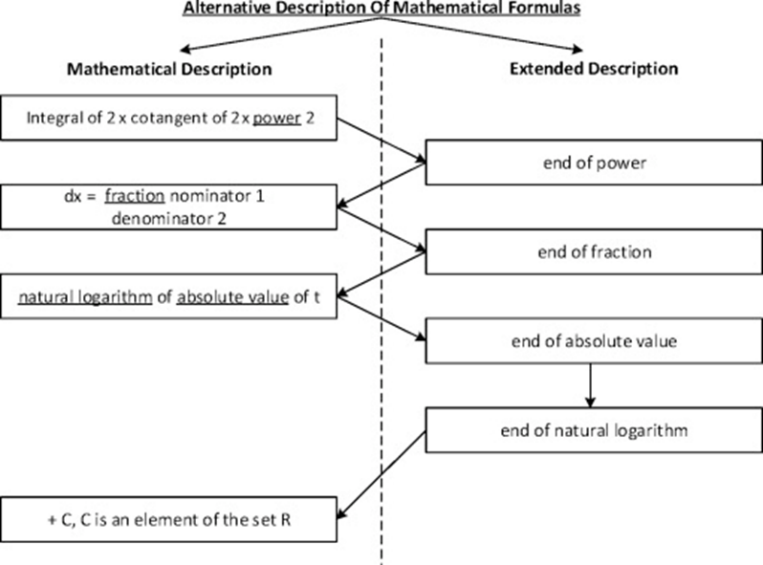
\includegraphics[width=5in]{./pics/1}
\caption{The schema of alternative description of mathematical equation}
\label{fig01}
\end{figure}

	There are other alternative methods used in mathematics to present charts and drawings in the accessible form such as: Talking Tactile Tablet. At our University IVEO device is used by impaired students \cite{viewplus}. Support Office for disabled students produces tactile drawings. The use of tactile drawings with audio descriptions in e-learning is difficult because of the limited number of available devices owned by disabled students. Taking into account this barrier, the presented method is focused on exercises without graphics, but containing math formulae. Additionally, in our method the exercises with simple graphics, have a simple alternative descriptions prepared according to image description guidelines \cite{diagram}.
	
	Based on the elaborated rules, alternative descriptions of all math formulae included in exercises on intelligent tutoring math platform were prepared. According to the experience gained during the preparation of 60 exercises, manually preparation time of alternative descriptions ranges from 2 to 5 h. Alternative descriptions were prepared according to math's formulae descriptions guideline elaborated by the authors. The correctness of the description was evaluated by mathematician together with blind students. During the research, the automatic generation of alternative description was taken into account by using Speech Rule Engine (SRE), which translates XML formulae into speech strings according to the rules that can be specified in an extended XPath (XML Path Language) syntax \cite{speech}. However, the following limitations encountered: limited support for various screen readers and magnifiers and support for English language only. Additionally, SRE supports only MathML notation. In our case, it requires conversion from LATEX notation and extension of the stack of used technologies \cite{Sorge:2016}. Some researchers report challenges during this conversion \cite{Wang:2015}. Due to this facts, we decided to prepare the alternative descriptions manually.
	
\begin{figure}[t]
\centering
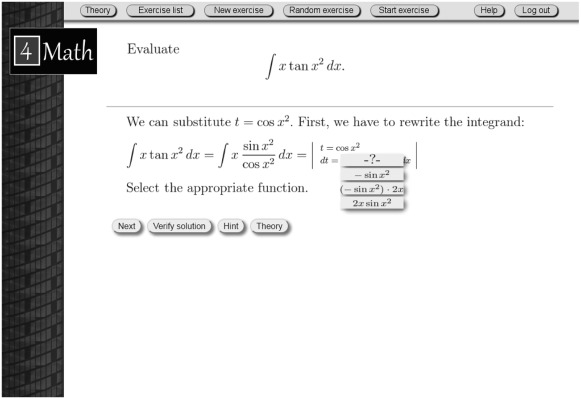
\includegraphics[width=5in]{./pics/2}
\caption{The schema of alternative description of mathematical equation}
\label{fig02}
\end{figure}

	Fig. \ref{fig03} below presents the alternative accessible presentation of equations (see section Methods for user interaction in Ref. \cite{Brzoza:2014}):
	
\begin{figure}[t]
\centering
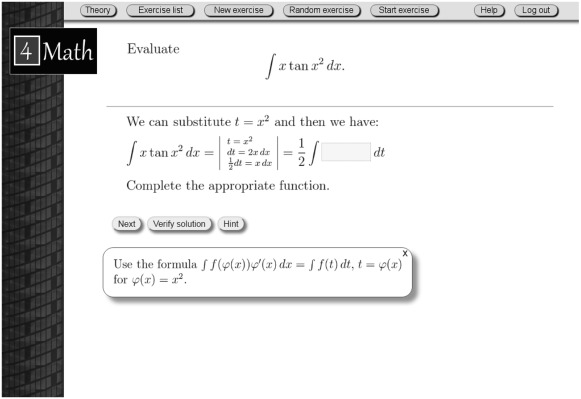
\includegraphics[width=5in]{./pics/3}
\caption{The example of exercize screen which allows the student to select the right integral function (the "Verify solution" path).}
\label{fig03}
\end{figure}

\begin{equation}
\label{eq1}
\int 2x \cot 2x2 dx = \ln | \sin 2x2 | + CC \in R
\end{equation}
	
	“Integral of 2× cotangent of 2× power 2 end of power dx = natural logarithm of absolute value of sine of 2× power 2 end of power end of absolute value end of natural logarithm + C, C is an element of the set R”

\begin{equation}
\label{eq2}
\int 2x \cot 2x2 dx = 12 \ln | \sin 2x2 | + CC \in R
\end{equation}
	
	“Integral of 2× cotangent of 2× power 2 end of power dx = fraction nominator 1 denominator 2 end of fraction natural logarithm of absolute value of sine of 2× power 2 end of power end of absolute value end of natural logarithm + C, C is an element of the set R”

\begin{equation}
\label{eq3}
\int 2x \cot 2x2 dx = -12 \ln | \cos x^2 | + CC \in R
\end{equation}

\begin{equation}
\label{eq4}
\int 2x \cot 2x^2 dx = 12 \ln | t | + CC \in R
\end{equation}

	Уach of the math formulae's alternative descriptions can be read interactively using assistive technology software such as Window-Eyes or Jaws \cite{window-eyes, job_access}. The screen readers allow for reading alternative description of entirely formula or read it by words or by characters. The alternative description of math formulae is included in the page content according to guideline for the aural rendering of a document prepared by The World Wide Web Consortium (W3C), which is already commonly used by the blind and print-impaired communities \cite{guideline}. Such an approach allows visually impaired student to resolve the exercise simultaneously and interactively with sighted student or teacher. The alternative description of mathematical formulae and interactive elements of user interface (text fields, drop-down lists, selection lists) for each exercise is stored in XML files.

\subsection{Implementation of the e-learning platforms for remote interactive mathematical education}
	Classical mathematics education for the blind is based on a combination of voice interaction with Braille mathematical notation. Usually, a teacher dictates an exercise verbally and a student writes the contents in the form of Braille. Next, the student solves the exercise and notes the following steps of the solution in Braille form. In the final step, the student reads aloud the obtained result to the teacher. Moreover, the indicated method requires individual work with the student.
	
	What is more, the voice message of both the student and the teacher needs to be refined, and it must clearly contain all the elements of mathematical notation. In fact, there are no standardized rules on reading mathematical formulae aloud.

	Fig. \ref{fig03} presents the exemplary exercise from the platform. A list of proposed solutions is given to the students and they are required to choose the correct option. They confirm their choice by pressing the Next button. When their answer is correct, the exercise is finished. If the answer is incorrect, the platform provides hints, guidance, theorems and math definition to help students \cite{Namahoe:2017}.
	
\begin{figure}[t]
\centering
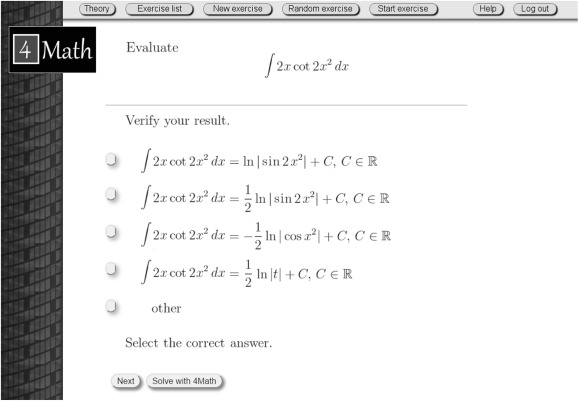
\includegraphics[width=5in]{./pics/4}
\caption{The example of exercise screen which allows the student to type the
correct value in the text field.}
\label{fig04}
\end{figure}

	In the exercise preparation phase, the method of interacting with a user is set. Figs. \ref{fig04} and \ref{fig05} present the exemplary screens. In Fig. \ref{fig05}, the user is required to write a correct value in the text field. Moreover, the user can use the hint button to display the additional helpful information. In Fig. \ref{fig05}, the way of interaction is based on choosing the correct answer from the drop-down list. For each presented graphical element an alternative text description is available. Moreover, the text is divided into small paragraphs for easier navigation, and it can be repeated selectively.

\subsection{Assessment methods}
	The developed solution brings new opportunities in the process of assessment of math skills by visually impaired people:

\begin{itemize}
	
	\item A more detailed history of activity related to the decoding of equations as well as the series of problems worked on by students with details of success, failure and support utilization,
    \item  The possibility of multiple repetition of the session (exercise solution) by the user – self assessment,
    \item  Automatic grouping the categories of mistakes made by students in resolving exercises (as mentioned earlier, mathematicians, who prepare exercises, define the dictionary of possible mathematical errors for every exercise),
    \item  Teacher's retrospective analysis of learning history for many visually impaired students without the knowledge of Braille notation.
\end{itemize}
	
\begin{figure}[t]
\centering
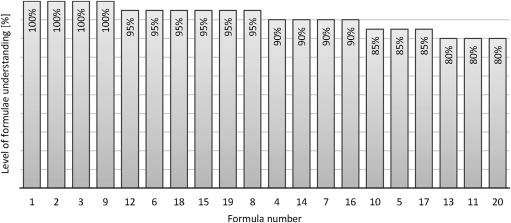
\includegraphics[width=5in]{./pics/5}
\caption{The example of exercise screen which allows the student to select the
correct answer from the drop-down list}
\label{fig05}
\end{figure}	
	
	Additionally, the platform implements the intelligent algorithms for automatic assessment of mathematics understanding. Based on the current assessment of the student's knowledge, the new exercises are proposed. The proposed algorithm that chooses exercise to solve it, takes into account the following criteria based on the history of previously solved exercises: the math area of exercise, the number of solved and not completely solved exercises, time of exercise solving, difficulty level, and possibility to make similar mistakes in new exercises. Our approach is based on adaptive testing algorithm to uncover latent knowledge. It based on hierarchical representation of all concept and knowledge with particular domain and knowledge vector, which represents the concepts that are understandable by a particular student \cite{Lynch:2014}.
	
	The teacher's role may be reduced to the choice of the session subject and assessment of the student's work in view of the number of: exercises solved by himself in a given time, errors made, hints used by the student to solve the selected exercises and others. Although the student's knowledge vector can be used by the teacher to explain the concepts that a student has not mastered yet.

\subsection{Evaluation of understanding an alternative description of mathematical formulae by blind students}
	The research was conducted among the group of 20 students (8 of them were blind and 12 of them were low vision). The students were selected from various schools and engineering university faculties. The age of the selected students range from 16 to 24 years. The criterion of inclusion was the fact that mathematics was completed at a mathematical college or technical university. The students were randomly assigned with 10 people in the control group (4 blind and 6 low vision) and 10 people in the experimental group (4 blind and 6 low vision). The mathematical skill between the two groups is considered comparable because everyone was familiar with the mathematical notation used in the tests. What is more the tests focused on understanding the notation of the formulae and did not require to solve them. The whole experiment was repeated twice. In the first attempt the control group used simple descriptions and the experimental group used alternative description of math structural information. The experiment concerned half of the mathematical formulae. In the second attempt the role of groups was switched and the second half of mathematical formulae were used.
	
	During the research, three groups of math formulae with an alternative description were prepared (which are included in the supplement):
	
	Simple formulae containing basic math operators such as: +, −, *, /, \textgreater, \textless, \%, numbers, variables, functions and brackets.
	
	Complex math formulae like simple formulae containing additionally two dimensional math structures such as fractions, roots, powers and nested two dimensional structures.
	
\begin{figure}[t]
\centering
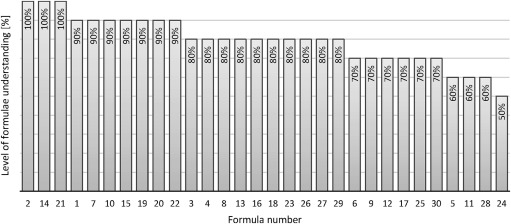
\includegraphics[width=5in]{./pics/6}
\caption{The level of simple formulae understanding by students}
\label{fig06}
\end{figure}	
	
	Advanced formulae like complex formulae containing additionally derivatives, integrals, limits, progressions and formulae from other areas of mathematics.
	
	The first and the second group contain respectively 20 formulae, and the last group contains 30 formulae. Each participant in the research was asked to fill the evaluation forms. The forms contained formula number, question about understanding the alternative description of the formula with two possible answers: good and poor, and the field for participant comment or suggestions.
	
	The formulae were read aloud by impaired students using their favourite assistive technologies screen readers such as: JAWS, Window Eyes or screen magnifiers with additional voice functions. It was possible to choose preferred speech synthesizer and its speech parameters such as: reading speed and voice pitch. The low visionstudents used the SuperNova or ZoomText MagReader. During the research, some of the students were observed by the math teachers who wrote additional comments about the way how students read interactively parts of the formulae.
\section{Results}
	
	Figs. \ref{fig06}-\ref{fig08} present the level of understanding the math formulae with alternative description of math structural information during the two phases of the experiment. Below each bar in the figures (the level of understanding) the formula number to which it relates is presented (see the supplement).
	
	According to Fig. \ref{fig06}, the level of simple math formulae understanding is 89\%. Some of the students had problem with understanding long formulae which contain many arguments and parenthesis. The example of such formula is presented in equation \ref{eq5}.

\begin{equation}
\label{eq5}
2x + (3x - 2) * (2x - 4) - 3x(4x - 1) = 0
\end{equation}

	During the second test, the students were asked to evaluate the complex formulae which additionally contained fractions, powers, roots and nested combination of such elements. It can be observed that understanding of the formulae which contained the nested two dimensional structures (fraction in fraction) were difficult for most of the students (result in Fig. \ref{fig07}). The example of such formula is presented in equation \ref{eq6}. Based on the teacher observation, it can be concluded that students had to read small parts of the formulae interactively many times to understand the meaning of the formula.

\begin{equation}
\label{eq6}
2x^x - 1x + 2 + x - 1x +2x^3 + 1 = 2x
\end{equation}

\begin{equation}
\label{eq7}
\int [ \cos - 2x\{1 - x\}] - 1 \log e{1+( \sin (2x(1-x^3)) \pi )}dx
\end{equation}

	The last group of testedontaining derivatives, integrals, limits, progressions and formulae from other areas of mathematics. The formulae were evaluated by ten students who study or graduated university math course. According to the research results presented in Fig. \ref{fig08} it can be concluded that formulae number 5, 11, 24, 28 were difficult to understand. The example of such formula is presented in equation \ref{eq7}. During the results analysis including students' comments, it can be stated that the nested two dimensional math structure with many parenthesis are the biggest problem in understanding such formulae. Some students informed also in the comments that they did not understand the evaluated formulae due to their insufficient higher mathematics knowledge.
\begin{table}[]
\caption{Attempts of experiments}
\label{experiments}
\centering
\resizebox{\textwidth}{!}{%
\begin{tabular}{|l|l|l|l|l|}
\hline
\begin{tabular}[c]{@{}l@{}}Simple \\ formulae \\ (structural \\ alternative \\ description)\end{tabular} & \begin{tabular}[c]{@{}l@{}}Complex \\ formulae\end{tabular} & \begin{tabular}[c]{@{}l@{}}Complex \\ formulae \\ (structural \\ alternative \\ description)\end{tabular} & \begin{tabular}[c]{@{}l@{}}Advanced \\ formulae\end{tabular} & \begin{tabular}[c]{@{}l@{}}Advanced \\ formulae \\ (structural \\ alternative \\ description)\end{tabular} \\ \hline
experimental group                                                                                       & control group                                               & experimental group                                                                                        & control group                                                & experimental group                                                                                         \\ \hline
87.5\%                                                                                                   & 40.0\%                                                      & 70.0\%                                                                                                    & 20.0\%                                                       & 70.0\%                                                                                                     \\ \hline
90.0\%                                                                                                   & 55.0\%                                                      & 80.0\%                                                                                                    & 50.0\%                                                       & 80.0\%                                                                                                     \\ \hline
92.5\%                                                                                                   & 82.5\%                                                      & 90.0\%                                                                                                    & 60.0\%                                                       & 90.0\%                                                                                                     \\ \hline
80.0\%                                                                                                   & 37.5\%                                                      & 70.0\%                                                                                                    & 12.5\%                                                       & 70.0\%                                                                                                     \\ \hline
90.0\%                                                                                                   & 50.0\%                                                      & 85.0\%                                                                                                    & 40.0\%                                                       & 85.0\%                                                                                                     \\ \hline
92.5\%                                                                                                   & 80.0\%                                                      & 90.0\%                                                                                                    & 60.0\%                                                       & 90.0\%                                                                                                     \\ \hline
\end{tabular}%
}
\end{table}

	The described experiments was repeated two times. Fig. \ref{fig09} presents the statistics of obtained results for first attempt of experiment. First the Shapiro–Wilk test is used to test of normality in frequentist statistics – it indicates no normal distribution. Then, the Wilcoxon test was used to demonstrate statistically significant difference in the level of understanding math formulae (p-values for performed inequality median tests are 0.0238, 0.0034, 4.1 × 10−8 for first attempt and 6.7 × 10−4, 3.3 × 10−4, 4.8 × 10−9 for second attempt respectively). The null hypothesis was that the median values of percent of formulae understanding in control and experimental group were no statistically significantly different. Because the results obtained during the second phase of the experiment (experiment 2 in Table \ref{experiments}) were similar to the first one, thus the authors decided to present the comparison between them in the form of the table. The results from both attempts of experiment are presented in Table \ref{experiments}.
	
\begin{figure}[t]
\centering
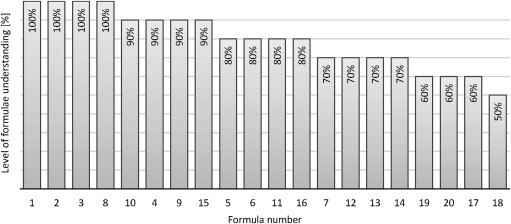
\includegraphics[width=5in]{./pics/7}
\caption{The level of complex formulae understanding by students (according to formula number in the supplement)}
\label{fig07}
\end{figure}		
	
\begin{figure}[t]
\centering
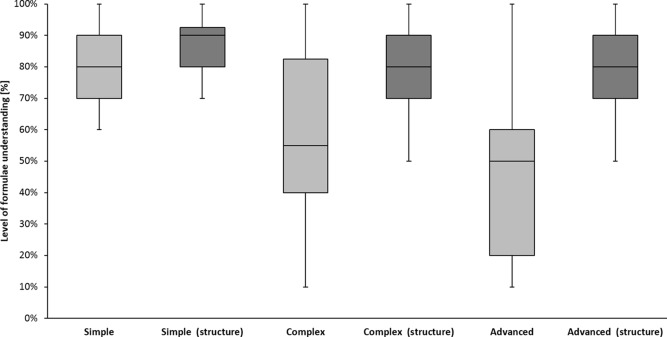
\includegraphics[width=5in]{./pics/8}
\caption{The level of advanced formulae understanding by students (according to formula number in the supplement)}
\label{fig08}
\end{figure}

\begin{figure}[t]
\centering
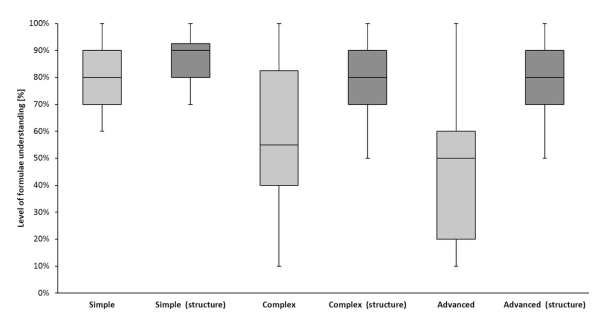
\includegraphics[width=5in]{./pics/9}
\caption{Distribution of the level of math formulae understanding for simple and structural alternative description during the first attempt of the experiment}
\label{fig09}
\end{figure}

	Regardless of the level of complexity of the math formulae the level of math formulae understanding is higher for alternative structural description. The difference to simple alternative description is proportional to the level of complexity of math formulae.
	
	The results of conducted research confirm a good understanding of math formulae described according to elaborated rules. Alternative descriptions of math formulae are also very helpful for low vision students that use screen magnifiers with additional voice functions.
	
	Currently, the 4Math platform is used in the process of education of approximately 1000 students and disabled students from six faculties at Silesian University of Technology. The platform includes three hundred of exercises from various branches of mathematical analysis with varying degrees of difficulty, of which about 30\% have been adapted for visually impaired people.
	
	After solving the adapted exercise they are able to achieve the required results which increase their chances for graduating. From the university point of view, it is beneficial that so many consultations between impaired students and the teacher are required. Comparing to the traditional math learning, where a student has to listen and make notes, the proposed method is focused on understanding the presented problem. Moreover, the platform is available during the entire high education. A student can return to math material and refresh a specific, currently needed knowledge.

\section{Discussion}
	The proposed solution eliminates the existing barriers in the process of teaching and assessment of mathematics for the blind. The main barrier was reported by Garderen et al., which is very little explicit instructional information about representations in the classical math text book \cite{Garderen:2012}. This main barrier is overcome in the presented method by introducing an additional feedback through the division of exercise mathematical propositions on elementary steps. This is much more than was introduced in the extension of the books for the blind (DAISY). The available tools for computer-aided learning mathematics, such as ALEKS \cite{Craiga:2013}, ActiveMath \cite{Goguadze:2005}, or MiniMatecaVox \cite{Henderson:2014}, do not allow for interactive solving exercises by blind students.
	
	The second important barrier is a cost of existing solutions. The authors in papers \cite{Brzoza:2012, Brzoza:2014} presented the alternative and graphic presentation of mathematical formulae using Braille and computer displays. However, it needs expensive Braille monitors.
	
	Generally, the presented approach increases the chance of higher education for the blind and also affects positively their self-esteem. The proposed solution can be used in the classroom with a teacher, but also as an e-learning platform.
	
	In order to adjust the platform to many national languages the specificity and diversity of them should be taken into account. Currently, there are no strictly specified rules for reading mathematical formulae in various languages. The similar problem exists because of the difference comparing between existing 6-point to national Braille notations and d 8-point mathematical Braille notation proposed in lambda project \cite{Brzoza:2012, Brzoza:2014}. In many cases, understanding the formulae while there are reading aloud requires the access to graphical presentation. For these reasons, a set of rules used for describing the structure of mathematical formulae should be designed to enable blind people understand them. It can be achieved by introducing additional vocabulary e.g. fraction, end of fraction, end of power etc. The designed learning platform contains tools (using XML notation, LaTeX as presentation format and a dedicated scripting language for interaction), which enable the preparation of courses with interactive exercises, and methods of their assessment. To summarize, the proposed method of interactive math problem solving, and alternative structural presentation can be easily adapted for another languages.
	
	Additionally, the proposed platform can be useful for preparing the interactive exercise covering different topics and subjects like physics, statistics and other technical courses.

\section{Conclusions}
	The tool for computer-aided interactive mathematics learning adapted to the needs of the blind has been designed, implemented and deployed as a platform for class and distance learning. This paper summarizes the experience of deploying it. The designed solution helps to overcome many barriers that occur in teaching impaired students. In the future it is intended to automate the process of adapting new math exercises.

\section{Summary}
	There are many problems with teaching and assessing impaired students in higher education, especially in technical science, where the knowledge is mostly represented by structural information like: math formulae, charts, graphs, etc. Developing e-learning platform for distance education solves this problem only partially due to the lack of accessibility for the blind.
	
	The proposed method is based on the decomposition of the typical mathematical exercise into a sequence of elementary sub-exercises. This allows the interactive resolving of math exercises and assessment of the correctness at every step. The presented method was prepared and evaluated by visually impaired people and students. The article presents tutoring platform for math teaching and assessment, and experience in exploring it by visually impaired people. During the research, three groups of math formulae with an alternative description were prepared:
\begin{itemize}
    \item Simple formulae containing basic math operators such as: +, -, *, /, \textgreater, \textless, \%, numbers, variables, functions and brackets.
    \item Complex math formulae like simple formulae containing additionally two-dimensional math structures such as fractions, roots, powers and nested two-dimensional structures.
    \item Advanced formulae like complex formulae containing additionally derivatives, integrals, limits, progressions and formulae from other areas of mathematics.
\end{itemize}

	The results of conducted research confirm a good understanding of math formulae described according to elaborated rules by blind people. Alternative descriptions are also very helpful for low vision students that use screen magnifiers with additional voice functions.
	
	Currently, the 4Math platform is used in the process of education of approximately 1000 students and disabled students from six faculties at Silesian University of Technology. The platform includes three hundred of exercises from various branches of mathematical analysis with varying degrees of difficulty, of which about 30\% have been adapted for visually impaired people.
	
	The designed solution helps to overcome many barriers that occur in teaching impaired students. In the future it is intended to automate the process of adapting new math exercises. Additionally, new rules of alternative presentation for exercises with graphical elements, such as charts and diagrams will be designed.

\section{Conflict of interest}
	There is no conflict of interest.

%\newpage
\section*{References}
\bibliographystyle{elsarticle-num}
\bibliography{my_bib}

\end{document}